
%% bare_jrnl.tex
%% V1.3
%% 2007/01/11
%% by Michael Shell
%% see http://www.michaelshell.org/
%% for current contact information.
%%
%% This is a skeleton file demonstrating the use of IEEEtran.cls
%% (requires IEEEtran.cls version 1.7 or later) with an IEEE journal paper.
%%
%% Support sites:
%% http://www.michaelshell.org/tex/ieeetran/
%% http://www.ctan.org/tex-archive/macros/latex/contrib/IEEEtran/
%% and
%% http://www.ieee.org/



% *** Authors should verify (and, if needed, correct) their LaTeX system  ***
% *** with the testflow diagnostic prior to trusting their LaTeX platform ***
% *** with production work. IEEE's font choices can trigger bugs that do  ***
% *** not appear when using other class files.                            ***
% The testflow support page is at:
% http://www.michaelshell.org/tex/testflow/


%%*************************************************************************
%% Legal Notice:
%% This code is offered as-is without any warranty either expressed or
%% implied; without even the implied warranty of MERCHANTABILITY or
%% FITNESS FOR A PARTICULAR PURPOSE! 
%% User assumes all risk.
%% In no event shall IEEE or any contributor to this code be liable for
%% any damages or losses, including, but not limited to, incidental,
%% consequential, or any other damages, resulting from the use or misuse
%% of any information contained here.
%%
%% All comments are the opinions of their respective authors and are not
%% necessarily endorsed by the IEEE.
%%
%% This work is distributed under the LaTeX Project Public License (LPPL)
%% ( http://www.latex-project.org/ ) version 1.3, and may be freely used,
%% distributed and modified. A copy of the LPPL, version 1.3, is included
%% in the base LaTeX documentation of all distributions of LaTeX released
%% 2003/12/01 or later.
%% Retain all contribution notices and credits.
%% ** Modified files should be clearly indicated as such, including  **
%% ** renaming them and changing author support contact information. **
%%
%% File list of work: IEEEtran.cls, IEEEtran_HOWTO.pdf, bare_adv.tex,
%%                    bare_conf.tex, bare_jrnl.tex, bare_jrnl_compsoc.tex
%%*************************************************************************

% Note that the a4paper option is mainly intended so that authors in
% countries using A4 can easily print to A4 and see how their papers will
% look in print - the typesetting of the document will not typically be
% affected with changes in paper size (but the bottom and side margins will).
% Use the testflow package mentioned above to verify correct handling of
% both paper sizes by the user's LaTeX system.
%
% Also note that the "draftcls" or "draftclsnofoot", not "draft", option
% should be used if it is desired that the figures are to be displayed in
% draft mode.
%
\documentclass[journal]{IEEEtran}
%
% If IEEEtran.cls has not been installed into the LaTeX system files,
% manually specify the path to it like:
% \documentclass[journal]{../sty/IEEEtran}





% Some very useful LaTeX packages include:
% (uncomment the ones you want to load)


% *** MISC UTILITY PACKAGES ***
%
%\usepackage{ifpdf}
% Heiko Oberdiek's ifpdf.sty is very useful if you need conditional
% compilation based on whether the output is pdf or dvi.
% usage:
% \ifpdf
%   % pdf code
% \else
%   % dvi code
% \fi
% The latest version of ifpdf.sty can be obtained from:
% http://www.ctan.org/tex-archive/macros/latex/contrib/oberdiek/
% Also, note that IEEEtran.cls V1.7 and later provides a builtin
% \ifCLASSINFOpdf conditional that works the same way.
% When switching from latex to pdflatex and vice-versa, the compiler may
% have to be run twice to clear warning/error messages.






% *** CITATION PACKAGES ***
%
\usepackage{cite}
% cite.sty was written by Donald Arseneau
% V1.6 and later of IEEEtran pre-defines the format of the cite.sty package
% \cite{} output to follow that of IEEE. Loading the cite package will
% result in citation numbers being automatically sorted and properly
% "compressed/ranged". e.g., [1], [9], [2], [7], [5], [6] without using
% cite.sty will become [1], [2], [5]--[7], [9] using cite.sty. cite.sty's
% \cite will automatically add leading space, if needed. Use cite.sty's
% noadjust option (cite.sty V3.8 and later) if you want to turn this off.
% cite.sty is already installed on most LaTeX systems. Be sure and use
% version 4.0 (2003-05-27) and later if using hyperref.sty. cite.sty does
% not currently provide for hyperlinked citations.
% The latest version can be obtained at:
% http://www.ctan.org/tex-archive/macros/latex/contrib/cite/
% The documentation is contained in the cite.sty file itself.






% *** GRAPHICS RELATED PACKAGES ***
%
\usepackage{graphicx}
\usepackage{pdfpages}
\usepackage{listings}
\usepackage{caption}
\usepackage{url}
% defines how code will be shown
\definecolor{dkgreen}{rgb}{0,0.6,0}
\definecolor{gray}{rgb}{0.5,0.5,0.5}
\definecolor{mauve}{rgb}{0.58,0,0.82}
% still code
\lstset{frame=tb,
  language=C, %Java
  aboveskip=3mm,
  belowskip=3mm,
  showstringspaces=false,
  columns=flexible,
  basicstyle={\small\ttfamily},
  numbers=none,
  numberstyle=\tiny\color{gray},
  keywordstyle=\color{blue},
  commentstyle=\color{dkgreen},
  stringstyle=\color{mauve},
  breaklines=true,
  breakatwhitespace=true
  tabsize=3
}

\ifCLASSINFOpdf
  %\usepackage[pdftex]{graphicx}
  % declare the path(s) where your graphic files are
  % \graphicspath{{../pdf/}{../jpeg/}}
  % and their extensions so you won't have to specify these with
  % every instance of \includegraphics
  % \DeclareGraphicsExtensions{.pdf,.jpeg,.png}
\else
  % or other class option (dvipsone, dvipdf, if not using dvips). graphicx
  % will default to the driver specified in the system graphics.cfg if no
  % driver is specified.
  % \usepackage[dvips]{graphicx}
  % declare the path(s) where your graphic files are
  % \graphicspath{{../eps/}}
  % and their extensions so you won't have to specify these with
  % every instance of \includegraphics
  % \DeclareGraphicsExtensions{.eps}
\fi
% graphicx was written by David Carlisle and Sebastian Rahtz. It is
% required if you want graphics, photos, etc. graphicx.sty is already
% installed on most LaTeX systems. The latest version and documentation can
% be obtained at: 
% http://www.ctan.org/tex-archive/macros/latex/required/graphics/
% Another good source of documentation is "Using Imported Graphics in
% LaTeX2e" by Keith Reckdahl which can be found as epslatex.ps or
% epslatex.pdf at: http://www.ctan.org/tex-archive/info/
%
% latex, and pdflatex in dvi mode, support graphics in encapsulated
% postscript (.eps) format. pdflatex in pdf mode supports graphics
% in .pdf, .jpeg, .png and .mps (metapost) formats. Users should ensure
% that all non-photo figures use a vector format (.eps, .pdf, .mps) and
% not a bitmapped formats (.jpeg, .png). IEEE frowns on bitmapped formats
% which can result in "jaggedy"/blurry rendering of lines and letters as
% well as large increases in file sizes.
%
% You can find documentation about the pdfTeX application at:
% http://www.tug.org/applications/pdftex





% *** MATH PACKAGES ***
%
%\usepackage[cmex10]{amsmath}
% A popular package from the American Mathematical Society that provides
% many useful and powerful commands for dealing with mathematics. If using
% it, be sure to load this package with the cmex10 option to ensure that
% only type 1 fonts will utilized at all point sizes. Without this option,
% it is possible that some math symbols, particularly those within
% footnotes, will be rendered in bitmap form which will result in a
% document that can not be IEEE Xplore compliant!
%
% Also, note that the amsmath package sets \interdisplaylinepenalty to 10000
% thus preventing page breaks from occurring within multiline equations. Use:
%\interdisplaylinepenalty=2500
% after loading amsmath to restore such page breaks as IEEEtran.cls normally
% does. amsmath.sty is already installed on most LaTeX systems. The latest
% version and documentation can be obtained at:
% http://www.ctan.org/tex-archive/macros/latex/required/amslatex/math/





% *** SPECIALIZED LIST PACKAGES ***
%
%\usepackage{algorithmic}
% algorithmic.sty was written by Peter Williams and Rogerio Brito.
% This package provides an algorithmic environment fo describing algorithms.
% You can use the algorithmic environment in-text or within a figure
% environment to provide for a floating algorithm. Do NOT use the algorithm
% floating environment provided by algorithm.sty (by the same authors) or
% algorithm2e.sty (by Christophe Fiorio) as IEEE does not use dedicated
% algorithm float types and packages that provide these will not provide
% correct IEEE style captions. The latest version and documentation of
% algorithmic.sty can be obtained at:
% http://www.ctan.org/tex-archive/macros/latex/contrib/algorithms/
% There is also a support site at:
% http://algorithms.berlios.de/index.html
% Also of interest may be the (relatively newer and more customizable)
% algorithmicx.sty package by Szasz Janos:
% http://www.ctan.org/tex-archive/macros/latex/contrib/algorithmicx/




% *** ALIGNMENT PACKAGES ***
%
%\usepackage{array}
% Frank Mittelbach's and David Carlisle's array.sty patches and improves
% the standard LaTeX2e array and tabular environments to provide better
% appearance and additional user controls. As the default LaTeX2e table
% generation code is lacking to the point of almost being broken with
% respect to the quality of the end results, all users are strongly
% advised to use an enhanced (at the very least that provided by array.sty)
% set of table tools. array.sty is already installed on most systems. The
% latest version and documentation can be obtained at:
% http://www.ctan.org/tex-archive/macros/latex/required/tools/


%\usepackage{mdwmath}
%\usepackage{mdwtab}
% Also highly recommended is Mark Wooding's extremely powerful MDW tools,
% especially mdwmath.sty and mdwtab.sty which are used to format equations
% and tables, respectively. The MDWtools set is already installed on most
% LaTeX systems. The lastest version and documentation is available at:
% http://www.ctan.org/tex-archive/macros/latex/contrib/mdwtools/


% IEEEtran contains the IEEEeqnarray family of commands that can be used to
% generate multiline equations as well as matrices, tables, etc., of high
% quality.


%\usepackage{eqparbox}
% Also of notable interest is Scott Pakin's eqparbox package for creating
% (automatically sized) equal width boxes - aka "natural width parboxes".
% Available at:
% http://www.ctan.org/tex-archive/macros/latex/contrib/eqparbox/





% *** SUBFIGURE PACKAGES ***
%\usepackage[tight,footnotesize]{subfigure}
% subfigure.sty was written by Steven Douglas Cochran. This package makes it
% easy to put subfigures in your figures. e.g., "Figure 1a and 1b". For IEEE
% work, it is a good idea to load it with the tight package option to reduce
% the amount of white space around the subfigures. subfigure.sty is already
% installed on most LaTeX systems. The latest version and documentation can
% be obtained at:
% http://www.ctan.org/tex-archive/obsolete/macros/latex/contrib/subfigure/
% subfigure.sty has been superceeded by subfig.sty.



%\usepackage[caption=false]{caption}
%\usepackage[font=footnotesize]{subfig}
% subfig.sty, also written by Steven Douglas Cochran, is the modern
% replacement for subfigure.sty. However, subfig.sty requires and
% automatically loads Axel Sommerfeldt's caption.sty which will override
% IEEEtran.cls handling of captions and this will result in nonIEEE style
% figure/table captions. To prevent this problem, be sure and preload
% caption.sty with its "caption=false" package option. This is will preserve
% IEEEtran.cls handing of captions. Version 1.3 (2005/06/28) and later 
% (recommended due to many improvements over 1.2) of subfig.sty supports
% the caption=false option directly:
%\usepackage[caption=false,font=footnotesize]{subfig}
%
% The latest version and documentation can be obtained at:
% http://www.ctan.org/tex-archive/macros/latex/contrib/subfig/
% The latest version and documentation of caption.sty can be obtained at:
% http://www.ctan.org/tex-archive/macros/latex/contrib/caption/




% *** FLOAT PACKAGES ***
%
%\usepackage{fixltx2e}
% fixltx2e, the successor to the earlier fix2col.sty, was written by
% Frank Mittelbach and David Carlisle. This package corrects a few problems
% in the LaTeX2e kernel, the most notable of which is that in current
% LaTeX2e releases, the ordering of single and double column floats is not
% guaranteed to be preserved. Thus, an unpatched LaTeX2e can allow a
% single column figure to be placed prior to an earlier double column
% figure. The latest version and documentation can be found at:
% http://www.ctan.org/tex-archive/macros/latex/base/



%\usepackage{stfloats}
% stfloats.sty was written by Sigitas Tolusis. This package gives LaTeX2e
% the ability to do double column floats at the bottom of the page as well
% as the top. (e.g., "\begin{figure*}[!b]" is not normally possible in
% LaTeX2e). It also provides a command:
%\fnbelowfloat
% to enable the placement of footnotes below bottom floats (the standard
% LaTeX2e kernel puts them above bottom floats). This is an invasive package
% which rewrites many portions of the LaTeX2e float routines. It may not work
% with other packages that modify the LaTeX2e float routines. The latest
% version and documentation can be obtained at:
% http://www.ctan.org/tex-archive/macros/latex/contrib/sttools/
% Documentation is contained in the stfloats.sty comments as well as in the
% presfull.pdf file. Do not use the stfloats baselinefloat ability as IEEE
% does not allow \baselineskip to stretch. Authors submitting work to the
% IEEE should note that IEEE rarely uses double column equations and
% that authors should try to avoid such use. Do not be tempted to use the
% cuted.sty or midfloat.sty packages (also by Sigitas Tolusis) as IEEE does
% not format its papers in such ways.


%\ifCLASSOPTIONcaptionsoff
%  \usepackage[nomarkers]{endfloat}
% \let\MYoriglatexcaption\caption
% \renewcommand{\caption}[2][\relax]{\MYoriglatexcaption[#2]{#2}}
%\fi
% endfloat.sty was written by James Darrell McCauley and Jeff Goldberg.
% This package may be useful when used in conjunction with IEEEtran.cls'
% captionsoff option. Some IEEE journals/societies require that submissions
% have lists of figures/tables at the end of the paper and that
% figures/tables without any captions are placed on a page by themselves at
% the end of the document. If needed, the draftcls IEEEtran class option or
% \CLASSINPUTbaselinestretch interface can be used to increase the line
% spacing as well. Be sure and use the nomarkers option of endfloat to
% prevent endfloat from "marking" where the figures would have been placed
% in the text. The two hack lines of code above are a slight modification of
% that suggested by in the endfloat docs (section 8.3.1) to ensure that
% the full captions always appear in the list of figures/tables - even if
% the user used the short optional argument of \caption[]{}.
% IEEE papers do not typically make use of \caption[]'s optional argument,
% so this should not be an issue. A similar trick can be used to disable
% captions of packages such as subfig.sty that lack options to turn off
% the subcaptions:
% For subfig.sty:
% \let\MYorigsubfloat\subfloat
% \renewcommand{\subfloat}[2][\relax]{\MYorigsubfloat[]{#2}}
% For subfigure.sty:
% \let\MYorigsubfigure\subfigure
% \renewcommand{\subfigure}[2][\relax]{\MYorigsubfigure[]{#2}}
% However, the above trick will not work if both optional arguments of
% the \subfloat/subfig command are used. Furthermore, there needs to be a
% description of each subfigure *somewhere* and endfloat does not add
% subfigure captions to its list of figures. Thus, the best approach is to
% avoid the use of subfigure captions (many IEEE journals avoid them anyway)
% and instead reference/explain all the subfigures within the main caption.
% The latest version of endfloat.sty and its documentation can obtained at:
% http://www.ctan.org/tex-archive/macros/latex/contrib/endfloat/
%
% The IEEEtran \ifCLASSOPTIONcaptionsoff conditional can also be used
% later in the document, say, to conditionally put the References on a 
% page by themselves.





% *** PDF, URL AND HYPERLINK PACKAGES ***
%
%\usepackage{url}
% url.sty was written by Donald Arseneau. It provides better support for
% handling and breaking URLs. url.sty is already installed on most LaTeX
% systems. The latest version can be obtained at:
% http://www.ctan.org/tex-archive/macros/latex/contrib/misc/
% Read the url.sty source comments for usage information. Basically,
% \url{my_url_here}.





% *** Do not adjust lengths that control margins, column widths, etc. ***
% *** Do not use packages that alter fonts (such as pslatex).         ***
% There should be no need to do such things with IEEEtran.cls V1.6 and later.
% (Unless specifically asked to do so by the journal or conference you plan
% to submit to, of course. )


% correct bad hyphenation here
%\hyphenation{op-tical net-works semi-conduc-tor}


\begin{document}
%
% paper title
% can use linebreaks \\ within to get better formatting as desired
\title{CSM6120 - 8 puzzle solver }
%
%
% author names and IEEE memberships
% note positions of commas and nonbreaking spaces ( ~ ) LaTeX will not break
% a structure at a ~ so this keeps an author's name from being broken across
% two lines.
% use \thanks{} to gain access to the first footnote area
% a separate \thanks must be used for each paragraph as LaTeX2e's \thanks
% was not built to handle multiple paragraphs
%

\author{Stefan Klaus, stk4@aber.ac.uk}

% note the % following the last \IEEEmembership and also \thanks - 
% these prevent an unwanted space from occurring between the last author name
% and the end of the author line. i.e., if you had this:
% 
% \author{....lastname \thanks{...} \thanks{...} }
%                     ^------------^------------^----Do not want these spaces!
%
% a space would be appended to the last name and could cause every name on that
% line to be shifted left slightly. This is one of those "LaTeX things". For
% instance, "\textbf{A} \textbf{B}" will typeset as "A B" not "AB". To get
% "AB" then you have to do: "\textbf{A}\textbf{B}"
% \thanks is no different in this regard, so shield the last } of each \thanks
% that ends a line with a % and do not let a space in before the next \thanks.
% Spaces after \IEEEmembership other than the last one are OK (and needed) as
% you are supposed to have spaces between the names. For what it is worth,
% this is a minor point as most people would not even notice if the said evil
% space somehow managed to creep in.






% If you want to put a publisher's ID mark on the page you can do it like
% this:
%\IEEEpubid{0000--0000/00\$00.00~\copyright~2007 IEEE}
% Remember, if you use this you must call \IEEEpubidadjcol in the second
% column for its text to clear the IEEEpubid mark.



% use for special paper notices
%\IEEEspecialpapernotice{(Invited Paper)}




% make the title area
\maketitle



\section{Structure}\label{sec:structure}
The overall structure can be seen in the UML diagram, found in appendix A though C.
In this section the structure of the program will be explained and the different classes and their uses. Detailed description methods will not be given please refer to the JavaDoc 
add the end of this document.
The structure of this section is as follows: for every package used in the program the use of the package as well as the classes inside it is given followed by a section about the justification of the design choices. 

\subsection{The csm6120 Package}\label{sec:csm6120Package}
This package holds the Main class, aswell as the \textit{State} and \textit{FileManager classes}. \\
The class diagram for this can be found in Appendix \ref{csm6120PackageUML} on page \pageref{csm6120PackageUML}.\\
This package acts as entry point to the program where the input files are read and where the \textit{State} class is located. \\

\subsubsection{Main}
The Main class is the entrance to the program. \\
The main method takes command line arguments such as the path to the start state and goal state of the puzzle(in .txt files) and a string which specifies what algorithm to use. \\
It creates instances of the FileManager object and State objects and calls the algorithm chosen by the user.\\

\subsubsection{State}
The State class holds variables and methods to manipulate and represent each state of the puzzle, that is the tile placement of the puzzle. \\
The tiles are interpreted as a simple arrayList, this has been done in order to make manipulating the array easier. \\
The class holds methods to switch 2 given tiles(done based on their index in the arrayList) as well as other common methods such as getters and methods to compare a state object to another. \\
These methods are used in the other algorithms incorporated in the program. \\

\subsubsection{FileManager}
The FileManager class holds methods to read input from a file, converts the strings into integers and then save it to the integer ArrayList in a State object. \\
The main class instantiates a single FileManager object and than uses it to read the input files provided by the user.\\

\subsubsection{Justification}
The idea for the \textit{csm6120 Package} was to have the methods which manipulate the input files all in one place. It was considered to move the State class to the \textit{SearchTree} package, but considering it holds such a central role in the program the decision fell against it. \\
The FileManager class was created in order to have a separate class to handle input files, this was done in order to follow object orientated design structures. \\

\subsection{The SearchTree Package}\label{sec:searchTreePackage}
This package holds classes which represent and generate the search tree.\\
The UML diagram for this can be found in appendix \ref{searchTreeUML} on page \pageref{searchTreeUML}\\

\subsubsection{TreeNode}
Objects of the TreeNode class represent nodes of the search tree. \\
Every TreeNode holds a State object as well as 2 linkedLists. One linkedList holding the children of one particular node, the other for holding its siblings. \\
The class has methods to add, get and remove nodes from those lists, as well as common methods such as returning if a list is empty. \\

\subsubsection{Graph}
The graph is used to generate the next step of the graph, by expanding all possible children from a particular TreeNode object and than add them to the linkedlist of children of said TreeNode object. \\
The nextStep method of this class checks where the empty tile is in a given TreeNode object, based on that it calls one of three possible functions which generate the children of the object. 

\subsubsection{Justification}
The idea was to have all classes which represent or manipulate the nodes of the search tree in a single package. It was also decided to only have a class for the nodes of the tree and representing the connections to its children using a internal linkedList rather than having a separate edge class which only links 2 nodes together. The reason this was done was for simplicity: using linkedList methods like adding and returning makes it easier considering every node has a very limited, maximum of 4, number of possible children. 

\subsection{SearchAlgorithm Package}\label{sec:searchAlgorithmPackage}
This package holds all search algorithms implemented in the program, as well as all supporting classes needed for them. \\
The UML diagram for this package can be seen in appendix \ref{searchAlgorithmUML} on page \pageref{searchAlgorithmUML}. \\

In general all the search algorithms are build up much the same way, they take 2 parameters: a start and goal State object, these States are than used to create the first node of the search tree, the goal state gets saved in the current search algorithm object and is used to check if the goal state of the puzzle has been reached. \\
The algorithms use the classes from the SearchTree package(see section \ref{sec:searchTreePackage}) to generate the search tree. \\ 
At the beginning of each algorithm it is checked if the start state is equal the goal state, this might be a rare occurrence but a useful functionality non the less. \\
All algorithms also hold a list of all previous expanded nodes, which all new generated nodes are checked against in order to prevent infinity loops. That already visited nodes are created again is because the children to each node are generated without knowledge if such a node has been created before, so infinity loops would be created relatively early on in the search trees. \\

\subsubsection{Breadth-First search}
This class holds the breadth-first search algorithm. \\
This algorithm works using a first-come first served queue. \\

\subsubsection{Depth-First search}
This class holds the depth-first search algorithm. \\
It is in its structure very similar to the breadth-first search algorithm, however uses a last-in first-out stack. \\

\subsubsection{Greedy Best-First search}
This class holds the greedy best-first search algorithm.\\
It is in its structure very like the breadth-first or depth-first algorithms, however uses a priority queue. In the priority queue the elements are sorted according to its \textit{natural ordering}, meaning from lower to higher numbers. \\
That way the treeNode which is closer to the goal state will be checked next. 
The priority queue uses the stateComparator class to sort its elements.\\

\subsubsection{A star algorithm}
This class holds the A star search algorithm.\\
This algorithm is similar to the greedy best-first algorithm in that it uses a priority queue, but it also uses a more advanced heuristic to decide which nodes to add to the queue in the first place. \\
This class holds 2 methods, one is the search algorithm in itself, the other is a method used to decide which treeNode object to add to the search queue. This is done using the Manhattan Distance heuristic. In the beginning of the algorithm the Manhattan Distance to the goal state is calculated and saved to a variable. \\
The addNode method than uses the current treeNode object and the goal State to calculate the Manhattan distance for each of the current treeNode's children. If the calculated Manhattan Distance is equal or less than the one calculated at the beginning of the algorithm the node is added to the search queue. Should the calculated distance be larger the child is discarded. \\
To calculate the Manhattan Distance the a ManhattanDistance object is used. \\

\subsubsection{StateComparator}
This class holds the StateComparator method used to compare to states in a priority list. This class implements the \textit{Comparator} interface. \\
It uses the String representation of a State objects state array to do the comparison. \\

\subsubsection{ManhattanDistance}
This class holds the methods used to calculate the Manhattan Distance. \\
During development of an early method to calculate the Manhattan Distance straight from a state array a number of problems have been found. The decision was made that a 2D representation of the array would be more fitting in order to calculate the Manhattan Distance. \\
However in order to avoid having to refactor all other algorithms the ManhattanDistance class holds methods to change an input arrayList to a simple array and after that to a 2 dimensional array. \\

The Manhattan Distance is calculated as such:\\
For each possible number of the puzzle find its index X and Y coordinates for each of the 2 input States. Then compare the X and Y coordinates of both indices and calculate the total difference in tiles. \\

Here 2 things must be nodded:\\
Depending on if the start State indices minus the goal State indices return a value less than zero or above, the formula gets flipped in order to prevent receiving a negative Manhattan Distance. The code for this is shown below:\\
\begin{lstlisting}
if (startArray[i][j] == goalArray[i][j]) {
	continue;
} else if (startArray[i][j] - goalArray[i][j] < 0) {
	manhattanDistanceSum += Math.abs(x_start - x_goal)
		+ Math.abs(y_start - y_goal);
} else if (startArray[i][j] - goalArray[i][j] > 0) {
	manhattanDistanceSum += Math.abs(x_goal - x_start)
		+ Math.abs(y_goal - y_start);
}
\end{lstlisting}

The other important thing to node is that empty/zero tile of the puzzle is ignored in the Manhattan Distance calculation, this is to accommodate the fact that at every iteration 2 tiles are switched.\\

\subsubsection{Justification}
It can be argued that the methods in the ManhattanDistance class are bad practice, as it would have been better to refactor all previously written algorithm to use 2D arrays rather than converting a State arrayList to a 2D array for every treeNode object. \\
However this decision was made as the use of a arrayList makes the use of the algorithms though out the program easier, thanks to Java's inbuilt arrayList methods. \\
Also since all arrayList have a limited size of 8, the computational cost for the conversion is constant and not large. \\

The list of expanded nodes which each class holds and all algorithms loop over at every iteration to check if the current nodes children already where created ones add a lot of computational overhead to each iteration. \\
While it gets apparent in breadth-first,however not as much in greedy best-first and A star search, this is not to much a problem because of the typical behaviour of these algorithms the overhead. But in depth-first search it causes massive computational overhead and causes long run times in order to find a solution. \\
The reason for that is the behaviour of the algorithm, unless in a few seldom instances the state space for depth-first search is much more massive than for the other algorithms. \\
So iterating over 10's of thousands of nodes in the list of expanded nodes takes a lot of time and computational power. \\
Still the list needs to be maintained in order to avoid infinite loop problems.


\section{Analysis}\label{sec:analysis}
In this section the design choices will be analysed further. \\
This includes the heuristic used as well as any problems encountered during the development cycle. \\

\subsection{Manhattan Distance}
For this program 2 heuristics where considered.\\
The first being simply the number of misplaced tiles, this heuristic is admissible as all misplaced tiles must be moved atleast once. \\
However it was decided to implement something more "advanced" in form of the Manhattan Distance heuristic, which is another common heuristic for these kind of problems\cite{russell2009artificial}. \\
The Manhattan Distance is admissible for this kind of problem as it either estimates the exact number of moves needed or underestimates the total path costs needed to find a solution. \\
The Manhattan Distance is calculated by the sum of the vertical and horizontal distances of between to tiles, because tiles can not move along diagonals. \\

\subsection{Performance}
In this section the performance of each algorithm with the test cases is analysed. \\
The test cases used in this section are shown in table \ref{tab:testCases}. 
Test cases 1 through 3 are the ones supplied with the assignment description, test case 4 through 6 have been randomly generated.\\

It is interesting to node that the processing time varies between runs. While on the first run it is often a lot higher, the processing time reduces in the following couple of runs. until it either gets stable or varies between 2 values. All running times shown in this section are taken after 5 runs as it then appears to be stable. \\

\begin{table}[h]
\renewcommand{\arraystretch}{1.3}
\centering
\caption{Test cases used to test the program}
\begin{tabular}{|c|c|}
\hline
\bfseries Test case number & \bfseries Test case representation \\\hline
   & 1 2 0 \\
 1 & 3 4 5 \\
   & 6 7 8 \\\hline
   & 1 2 5 \\
 2 & 3 0 4 \\
   & 6 7 8 \\\hline
   & 3 2 0 \\
 3 & 6 1 5 \\
   & 7 4 8 \\\hline
   & 1 7 6 \\
 4 & 3 6 2 \\
   & 4 0 8 \\\hline   
   & 2 0 7 \\
 5 & 4 5 3 \\
   & 6 1 8 \\\hline
   & 7 4 1 \\
 6 & 2 8 0 \\
   & 5 6 3 \\\hline 
\end{tabular}
\label{tab:testCases}
\end{table}

\subsubsection{Breadth-First search}
Table \ref{tab:bfs} shows the performance of Breadth-First search.\\
As the test result show the number of explored nodes increases significantly when more tiles are out of place. The processing time also increases.\\
While during test cases 1 - 3 the number of expanded nodes and the actual path cost to the goal, as well as the processing time, increases marginally from the easiest test case(1) to the more advanced one(3), the path cost, number of expanded nodes as well as the running time increases drastically when solving the randomly generated puzzle, represented as test case 4 - 6. \\ 
\begin{table}[h]
\renewcommand{\arraystretch}{1.3}
\centering
\caption{Performance of Breadth-First Search}
\begin{tabular}{|c|c|c|c|}
\hline
\bfseries Test case &\bfseries Path Cost & \bfseries Expanded Nodes & \bfseries Running Time \\
 & & &  \bfseries in nanosecond\\\hline
1 & 3 & 7 & 5 \\
2 & 29 & 53 & 7\\
3 & 67 & 114 & 11 \\
4 & 58375 & 80176 & 90107\\
5 & 74135 & 94765 & 154391 \\
6 & 156672 & 169194 & 964196 \\\hline
\end{tabular}
\label{tab:bfs}
\end{table}


\subsubsection{Depth-First search}
Table \ref{tab:dfs} shows the performance of Depth-First search.\\
As can be seen the path cost is massive, a lot more than the in any other search algorithm implemented in the system. As well is the processing time. The reason for the immense path cost and processing time is the way children are added to nodes in the program, in combination with the working of Depth-First search. \\
It is likely that if nodes where added in a different way the path cost and processing time decrease. It could also be improved with implementing an abbreviation of Depth-First search, such as Depth-Limited search. \\
It is worth noting that the arguably more complex systems of Test Case 2, 3 and 4 actually have a lower path cost and lower computational time than the first one, where only 3 tiles are out of place. In fact test case 6 which is by far the most advanced puzzle is the fastest to be solved, while test case 5 which is the next most advanced has the longest processing time and highest path cost of all puzzles. \\

Even though Depth-First search has by far the most worst time and space complexity of all the implemented algorithms, however it is bound to find a solution to the problem since the search space is finite, however in the absolute worst case the performance of Depth-First search would be equal to a simple brute force approach.  \\

\begin{table}[h]
\renewcommand{\arraystretch}{1.3}
\centering
\caption{Performance of Depth-First Search}
\begin{tabular}{|c|c|c|c|}
\hline
\bfseries Test case &\bfseries Path Cost & \bfseries Expanded Nodes & \bfseries Running Time \\\
 & & &\bfseries in nanosecond\\\hline
1 & 169022 & 180688 & 1303747 \\
2 & 139063 & 175713 & 1115838 \\
3 & 111950 & 166823 & 895815 \\
4 & 112545 & 167212 & 854431 \\
5 & 176779 & 181273 & 1307069 \\
6 & 77218 & 132209 & 441747 \\\hline
\end{tabular}
\label{tab:dfs}
\end{table}

\subsubsection{Greedy Best-First search}
Table \ref{tab:gbfs} shows the performance of the Greedy Best-First search algorithm. \\
As the table shows, in the first and easiest test case the algorithm performs with perfect accuracy, choosing the direct path to the goal state. \\
Test case 2 and 3 as well show a large improvement in path cost over Depth-First search, however shows shows, in some cases, worse performance than Breadth-First search. It can be seen that the extra computational overhead of sorting the priority queue causes the algorithm to perform marginal slower than Breadth-First search.\\
Also does the simple heuristic used in this algorithm not guarantee a better solution to the, as for test cases 2 and 3 the path cost and the number of expanded nodes is,though only minimal, larger than Breadth-First search. \\
It shows however that using a heuristic for more advanced search problems, represented here as test cases 4 - 6, leads to far better performance than using an uninformed search. \\
\begin{table}[h]
\renewcommand{\arraystretch}{1.3}
\centering
\caption{Performance of Greedy Best-First search}
\begin{tabular}{|c|c|c|c|}
\hline
\bfseries Test case &\bfseries Path Cost & \bfseries Expanded Nodes & \bfseries Running Time \\
 & & &\bfseries in nanosecond\\\hline
1 & 2 & 5 & 6 \\
2 & 8 & 16 &7 \\
3 & 72 & 117 &19 \\
4 & 946 & 1379 & 100 \\
5 & 950 & 1385 & 167 \\
6 & 5259 & 7345 & 1378 \\\hline
\end{tabular}
\label{tab:gbfs}
\end{table}

\subsubsection{A star search}
Table \ref{tab:astar} shows the performance of the $A^*$ Algorithm.\\
Different in this table compared to the previous once is that an extra column has been added in to show the Manhattan Distance value which was calculated at the beginning of the algorithm. \\
As the table shows for test cases 1 and 2 the estimated Manhattan Distance was reached precisely. On test case 3 the algorithm had to explore 21 nodes in order to find the goal state, while the estimated Manhattan Distance was 6 notes. This shows that the heuristic is admissible as it does not overestimate the path cost. \\
The processing time is similar to Greedy Best-First and Breadth-First search. Even for the more advanced puzzle(test case 3). \\

However test case 4 \& 5 show that a good heuristic does not always leads to a goal state. \\
No solution could be found for these test cases, however the Manhattan Distance is estimated to be 11 in both. \\
As the other test case work fine there is no reason to believe that the algorithm itself it faulty, but rather that $A^*$ simply is not able to find a solution to every puzzle. \\
Test case 6 is by far the most difficult puzzle to solve and here even $A^*$ needs multiple thousand steps to find a solution.\\


\begin{table}[h]
\renewcommand{\arraystretch}{1.3}
\centering
\caption{Performance of A star search}
\begin{tabular}{|c|c|c|c|c|}
\hline
\bfseries Test case & \bfseries Manhattan & \bfseries Patch cost & \bfseries Expanded nodes & \bfseries Running Time \\
 &\bfseries Distance & & &\bfseries in nanosecond\\\hline
1 & 2 & 2 & 4 & 6 \\
2 & 4 & 4 & 7 & 7 \\
3 & 6 & 21 & 28 & 11\\ 
4 & 11 & / & / &  5 \\
5 & 11 & / & /& 6 \\
6 & 17 & 4879 & 6789 & 1206 \\\hline
\end{tabular}
\label{tab:astar}
\end{table}

\subsection{Problems}
In this subsection the problems encountered in the development cycle are discussed, as well as how they were solved.\\

\subsubsection{Infinite loop}
Early during the development process, after implementing Breadth-First and Depth-First search, a problem with the graph generation was encountered. The problem was that states which were already encountered got generated again. \\
The reason for was that no method was implemented to check if nodes were already generated. This led to infinite long search trees.\\ 

\begin{lstlisting}[caption= Solution to the Infinite Search Tree Problem , ,label=listing:expandedCheck]
while (node.childrenIsEmpty() != true) {
	/*
	 Add the current node to a an ArrayList of expanded nodes
	 */
	if (expanded.contains(node.getState().
			getStringtoString()) == false) {
		expanded.add(node.getState().
			getStringtoString());
	}
	String s = node.peekChild().getState().
		getStringtoString();
	if (expanded.contains(s) == false) {
		expanded.add(s);
		searchQueue.add(node.getFirstChild());
	} else {
		node.removeFirstChild();
	}
}
\end{lstlisting}

The solution to that is shown in listing \ref{listing:expandedCheck}. \\
With these few lines of code all expanded nodes are saved to a arrayList of expanded nodes, which than gets iterated through every iteration to check if a newly generated state already exists. If it does not the state will be added to the search queue/stack as well as to the list of expanded nodes. \\
This piece of code, although modified in case of the $A^*$ algorithm, is included in all algorithms. \\

This also led to improvement in the Breadth-First search algorithm. While the algorithm is complete, i.e. it is bound to find a solution in a finite search environment, but as already said the way states are generated in the algorithm leads to reoccurring states.\\
The implementation of this routine in the Breadth-First algorithm lead to improvements of path cost and expanded nodes. The path cost for test case 2 was reduces from 97 to 29 nodes and for test case 3 from 381 nodes to 67 nodes.\\

\subsubsection{Implementation of the Manhattan Distance heuristics}
The way the states of the puzzle was represented in this program caused problems when trying to calculated the Manhattan Distance used in the $A^*$ algorithm. \\
The states were hold in a standard Java ArrayList, this caused however problems when calculating the distance.\\ 
This was, already mentioned in section \ref{sec:structure}, by implementing a new class which converts the arrayList to a 2 dimensional array and then use the X and Y coordinates to calculate how much each tile had to move.\\
This was a problem because it took a while until it was realised that an arrayList makes it more difficult to calculate the Manhattan distance and after that how to get the algorithm for the Manhattan distance set up. A thread on stack overflow helped with finding a solution for that. The thread can be found using the URL in the footnote. \footnote{\url{http://tinyurl.com/nullh9d}}

\section{Discussion}
Section \ref{sec:analysis} shows the analysis of each algorithm and its performance on each of the test cases. \\
Inherently one could see it as a comparison of uninformed search VS informed search, with 2 examples for each type of search. It shows that for simple puzzles uninformed search methods perform equally well or better than some informed search algorithms, both in time and space complexity. It is however on the more advanced puzzles that the informedness of an heuristic shows an drastic improvement over uninformed strategies. \\
It also shows that an advanced heuristic can both perform better or worse than a simple heuristic. An example of that would be a direct comparison of Greedy Best-First vs $A^*$ search. $A^*$ uses a more advanced heuristic which leads to better results in the most test cases but it fails to find a solution for some cases. \\ 
 
The attributes of the algorithm play a big role as well. Depth-First search has very large time and space complexity, but is still guaranteed to find a solution as the search space is finite. Breadth-First search performs much better in every test case, however in the worst case scenario it would have the same time and space complexity as Depth-First search.\\ 
Greedy Best-First performs better for some test cases however has for the simplest puzzles worse time complexity. $A^*$ has the best time and space complexity of all algorithms implemented in this program however, as already mentioned, fails to find a solution for some of the more advanced test cases. Whereas the other algorithms, even depth-first search, find a solution. \\

While it gets quite apparent that the uninformed search methods can find solutions, the informed search algorithms perform better and are generally a better choice for these kind of problems. The performance of uninformed search strategies could be tested further with implementation of algorithms such as iterative deepening, which would greatly improve on Depth-First search, which is currently not much more than a brute force approach.

\section{Conclusion}
The test results delivered by the program show informed search strategies perform generally better than uninformed search strategies, even though uninformed search can find solutions faster for simple problems. \\
It would be interesting to implement further search search algorithms such as Iterative Deepening and Bidirectional search in the future and compare their results to that of the other algorithms. \\
Given more time it would also have been interesting to implement more advanced heuristics for $A^*$ and see how different heuristics can lead to different solutions.


% references section

% can use a bibliography generated by BibTeX as a .bbl file
% BibTeX documentation can be easily obtained at:
% http://www.ctan.org/tex-archive/biblio/bibtex/contrib/doc/
% The IEEEtran BibTeX style support page is at:
% http://www.michaelshell.org/tex/ieeetran/bibtex/
\bibliographystyle{IEEEtran}
% argument is your BibTeX string definitions and bibliography database(s)
%\bibliography{IEEEabrv,../bib/paper}


\bibliography{IEEEabrv,citations}




% if have a single appendix:
%\appendix[Proof of the Zonklar Equations]
% or
%\appendix  % for no appendix heading
% do not use \section anymore after \appendix, only \section*
% is possibly needed

% use appendices with more than one appendix
% then use \section to start each appendix
% you must declare a \section before using any
% \subsection or using \label (\appendices by itself
% starts a section numbered zero.)
%


\appendices
\newpage
\onecolumn

\section{csm1620 Package UML}\label{csm6120PackageUML}

\begin{figure}[h]
\centering
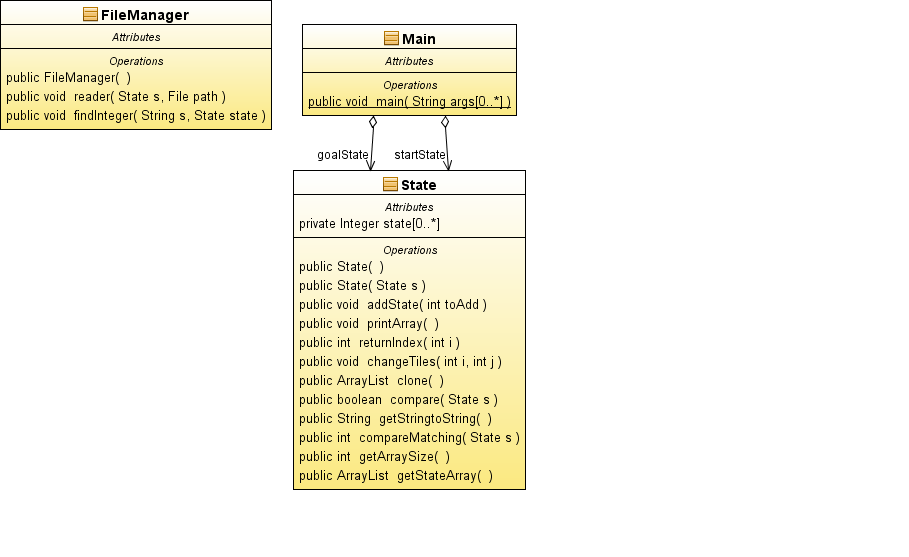
\includegraphics[width=1.4\textwidth,natwidth=610,natheight=642]{../Model/CSM6120_Assignment2-Model/ClassDiagram1.png} 

\end{figure}

\newpage
\section{SearchTree Package UML}\label{searchTreeUML}
\begin{figure}[h]
\centering
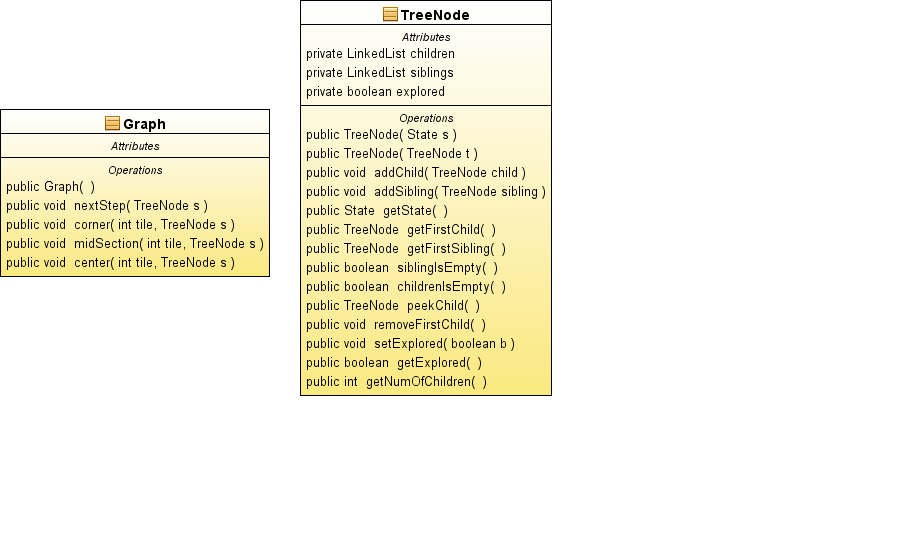
\includegraphics[width=1.4\textwidth,natwidth=610,natheight=642]{../Model/CSM6120_Assignment2-Model/ClassDiagram3.png} 

\end{figure}

% you can choose not to have a title for an appendix
% if you want by leaving the argument blank
\newpage
\section{SearchAlgorithm Package UML}\label{searchAlgorithmUML}
\begin{figure}[h]
\centering
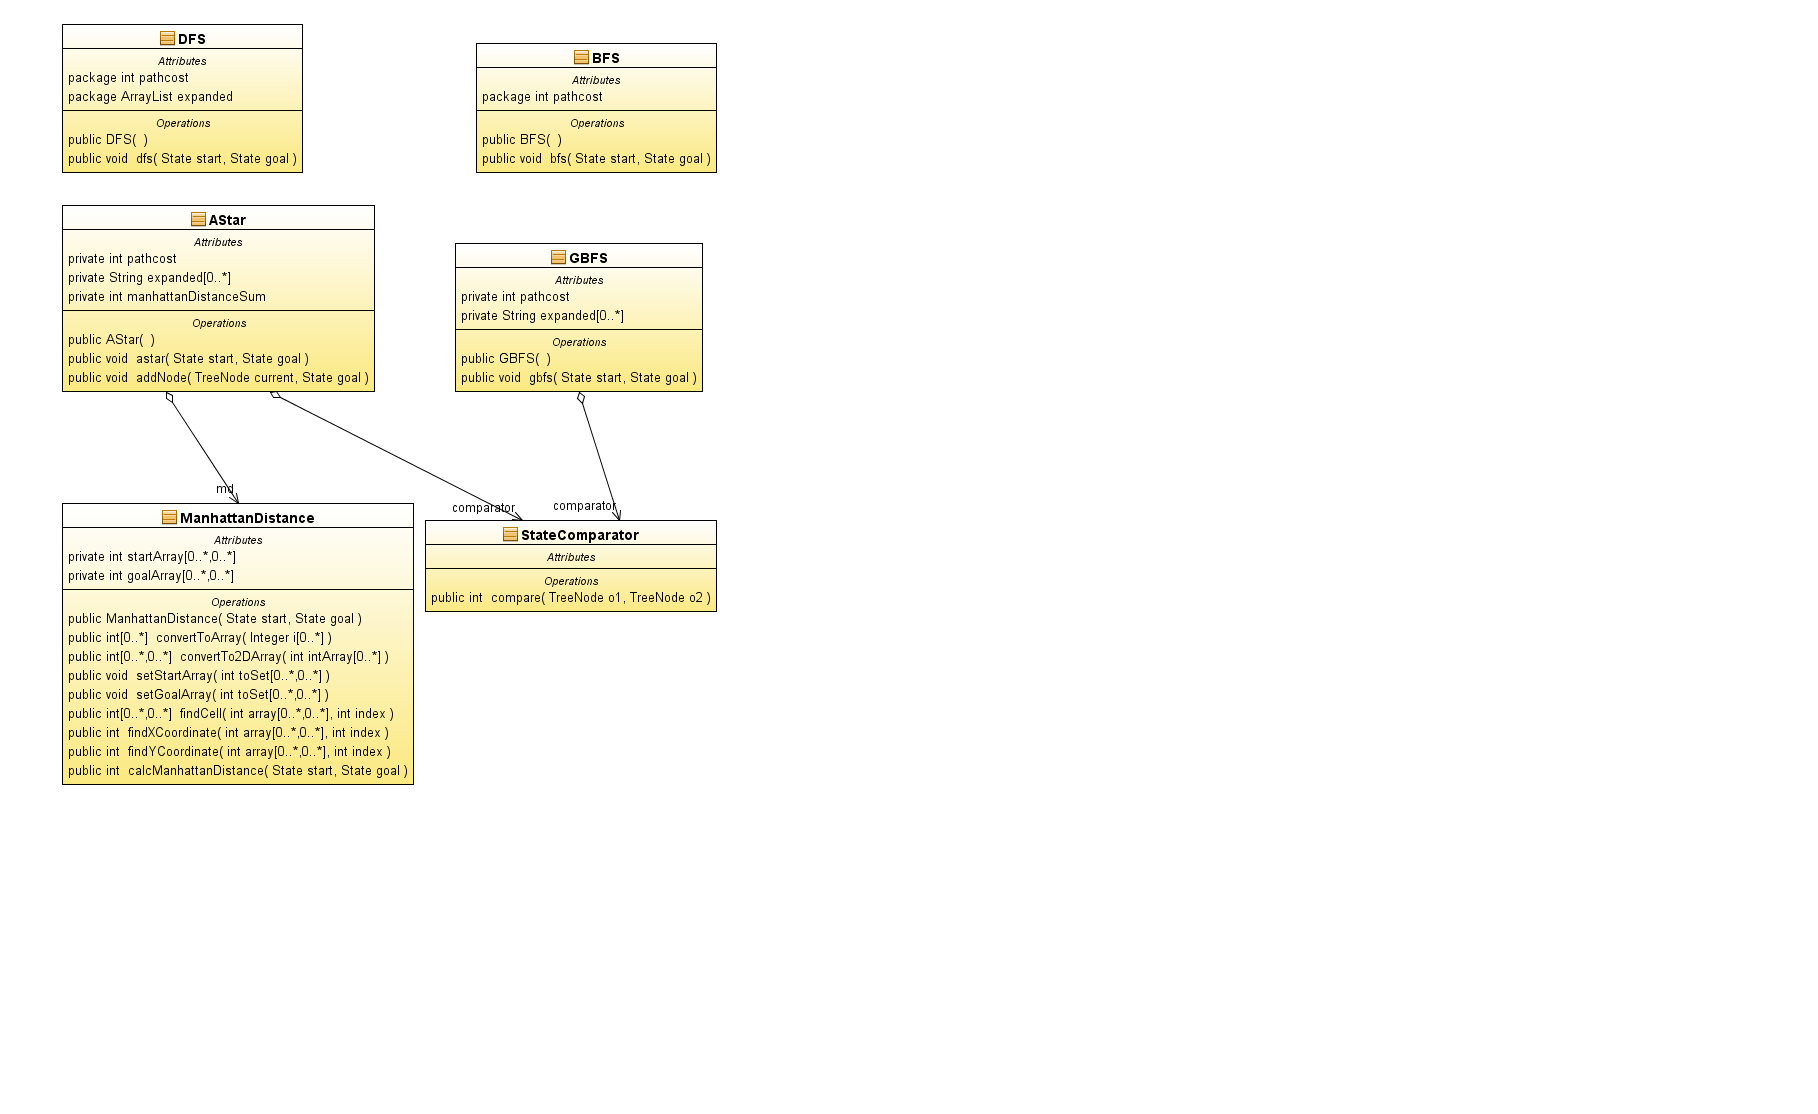
\includegraphics[width=1.6\textwidth,natwidth=610,natheight=642]{../Model/CSM6120_Assignment2-Model/ClassDiagram2.png} 

\end{figure}

\newpage
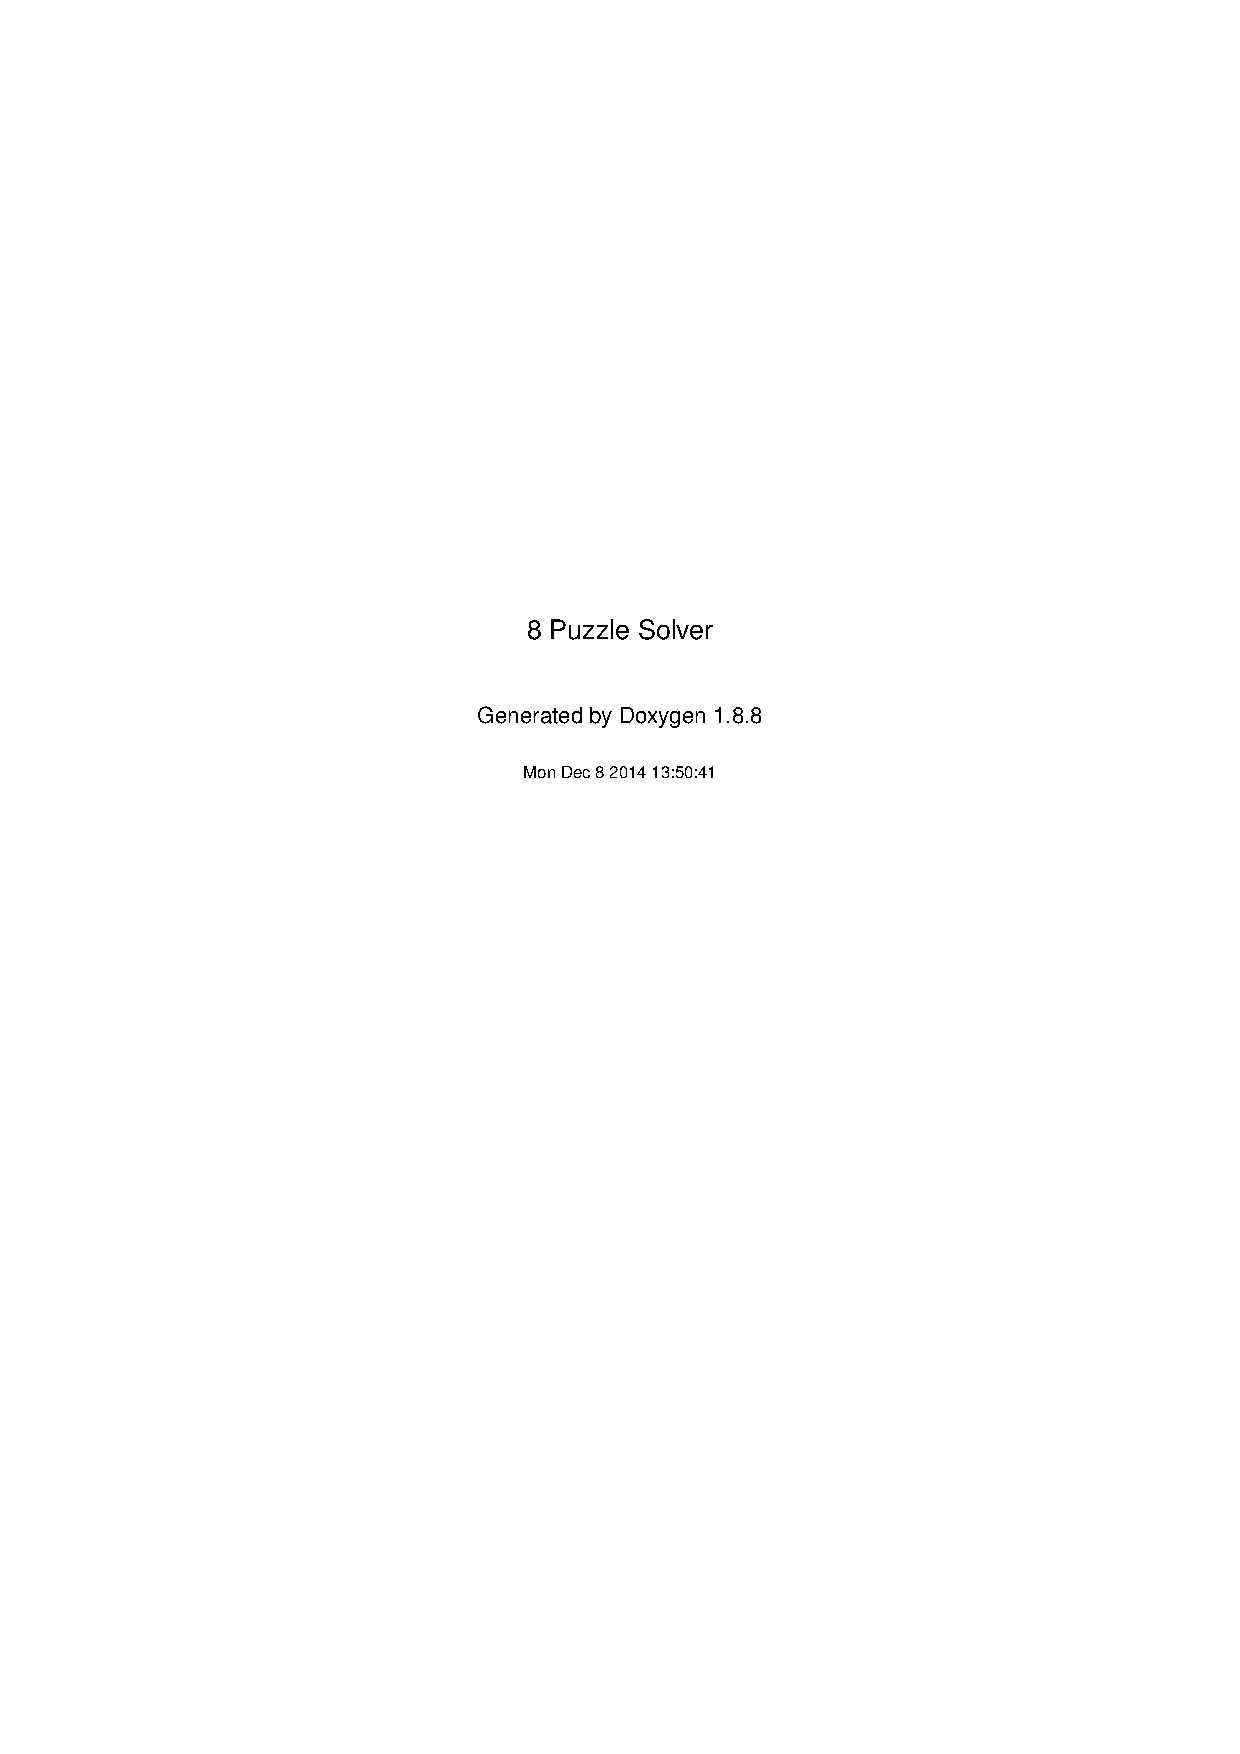
\includepdf[pages={1-}]{../JavaDoc/latex/refman.pdf}
%\includepdfmerge{../JavaDoc/latex/refman}
\twocolumn




% that's all folks
\end{document}


